% !TEX TS-program = pdflatex
% !TEX encoding = UTF-8 Unicode

\documentclass[a4paper, 13pt]{article} % A4 형식 및 글자 크기


% layout/spacing related packages
\usepackage[margin=0.5in]{geometry}
\usepackage{indentfirst} \parindent=1em	% 들여쓰기
\usepackage{microtype}
\usepackage{kotex}	% 한글 사용 가능
\usepackage{graphicx}
\usepackage{setspace} \onehalfspacing

\title{CapacityManger 소프트웨어 메뉴얼}

\author{문철승, 임동민, 황연수} 

\begin{document}
	
	\LARGE \maketitle
	
	\clearpage
	
	\normalsize
	\section{소프트웨어 선택 이유}
	본 소프트웨어를 선택한 이유는 컴퓨터 내 자료를 정리하지 않고 무분별하게 저장하여 사용하는 유저들의 자료 정리를 효율적으로 하기 위한 프로그램 중 인터페이스가 가장 단순하면서도 효과적인 사용이 가능하기 때문입니다.
	\section{소프트웨어 개요}
	본 소프트웨어는 사용자들의 컴퓨터에 존재하는 파일들(ex. 동영상, 이미지, 문서 등)의 위치를 파악하여 삭제 및 관리를 용이하게 할 수 있도록 도와주는 소프트웨어 입니다.
	\section{소프트웨어 사용}
	다음은 소프트웨어에 대한 설명이다.  실행창에는  \textbf{검사시작, 환경설정}버튼도있고,  \textbf{파일종류별로 볼수있는 창}(동영상,이미지,문서,기타)이 있다. 
		\subsection{exe실행파일 실행화면}
		크게 \textbf{검색시작, 환경설정 ,파일종류(동영상,이미지,문서,기타)}를 볼수 있다.
		검색시작을 누르면 파일 추출후 검색을 시작한다.
	\begin{figure}[h]
		\centering
		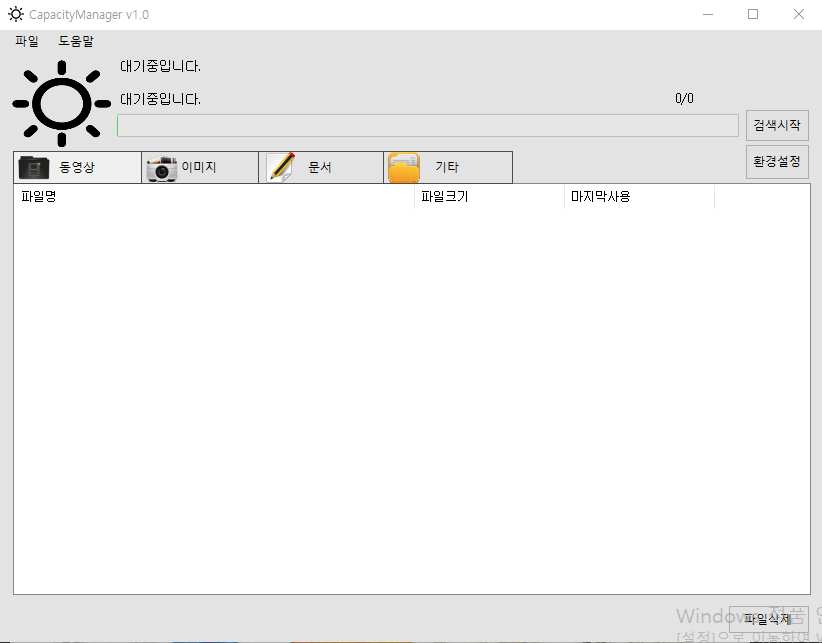
\includegraphics[width=0.7\textwidth]{Figures/exe2}
		\caption{exe실행파일 실행화면}
		\label{fig:exe2}
	\end{figure}

		\subsection{파일의 catalog}
		파일의 종류에는 \textbf{동영상,이미지,문서,기타}로 구분되어진다.
	\begin{figure}[h]
		\centering
		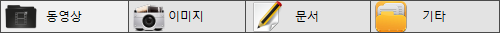
\includegraphics[width=0.7\textwidth]{Figures/catalog}
		\caption{catalog }
		\label{fig:catalog}
	\end{figure}

		\subsection{검색 완료창}
		검색이 완료된후 \textbf{파일저장위치,파일명, 파일크기, 최근사용일}로 구분되어 파일이 정리되어 뜬다.
		그외에도 총 파일 검사한수도 함께 뜬다.
	\begin{figure}[h]
		\centering
		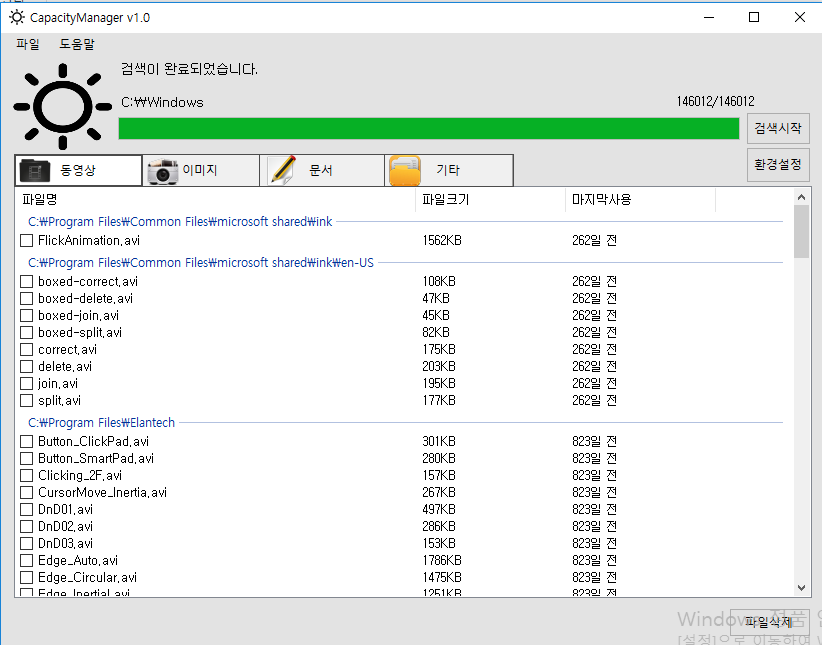
\includegraphics[width=0.7\textwidth]{Figures/complete}
		\caption{complete}
		\label{fig:complete}
	\end{figure}
		\subsection{catalog종류별}
		보기와 같이 \textbf{파일위치,파일명,크기,최근사용일},이 뜬다. 
	\begin{figure}[h]
		\centering
		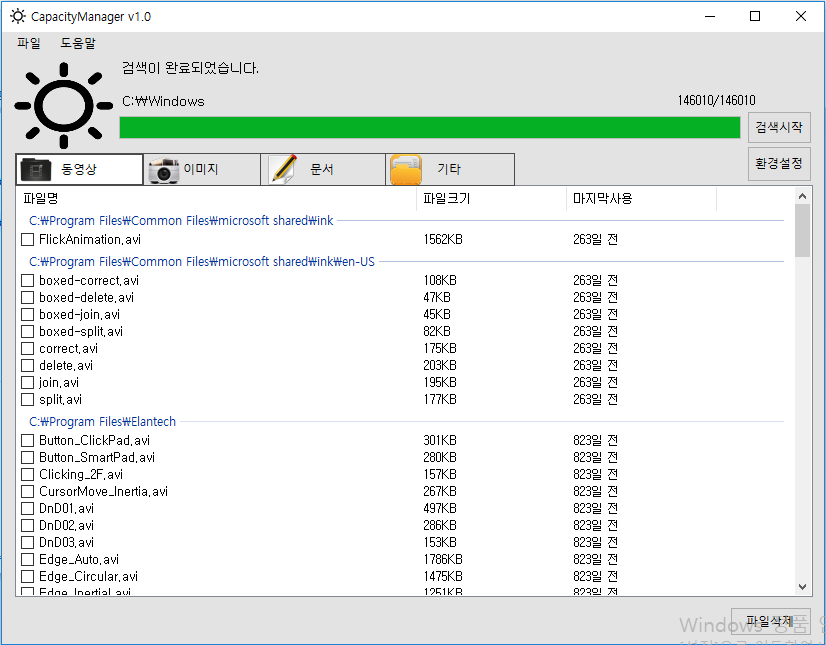
\includegraphics[width=0.7\textwidth]{Figures/avi}
		\caption{catalog: 동영상}
		\label{fig:avi}
	\end{figure}
	\begin{figure}[h]
		\centering
		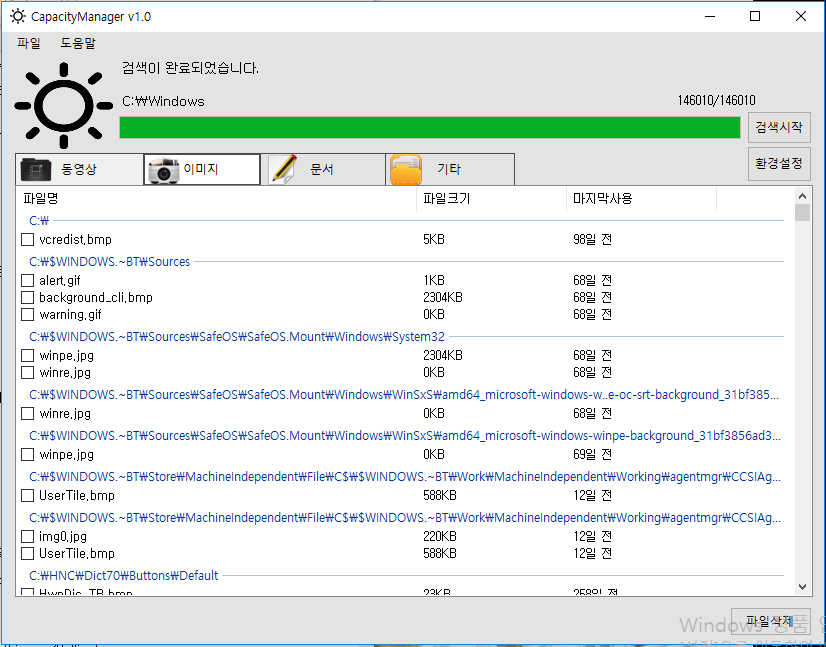
\includegraphics[width=0.7\textwidth]{Figures/jpg}
		\caption{catalog: 이미지}
		\label{fig:jpg}
	\end{figure}
	\section{환경설정}
	다음은 환경설정에 대한 설명이다.	환경설정은 크게 \textbf{검색폴더 선택, 동영상 확장자, 이미지 확장자, 문서 확장자, 기타 확장자, 검사예외 폴더, 최종 사용일자 설정} 등으로 나뉘어져 있다.
	
	검색폴더 선택칸을 제외하고 확장자 추가/삭제 버튼을 통해 \textbf{확장자를 변경한 후 확인 버튼을 누르면 변경된 값이 저장}된다.
	
	\begin{figure}[h]
		\centering
		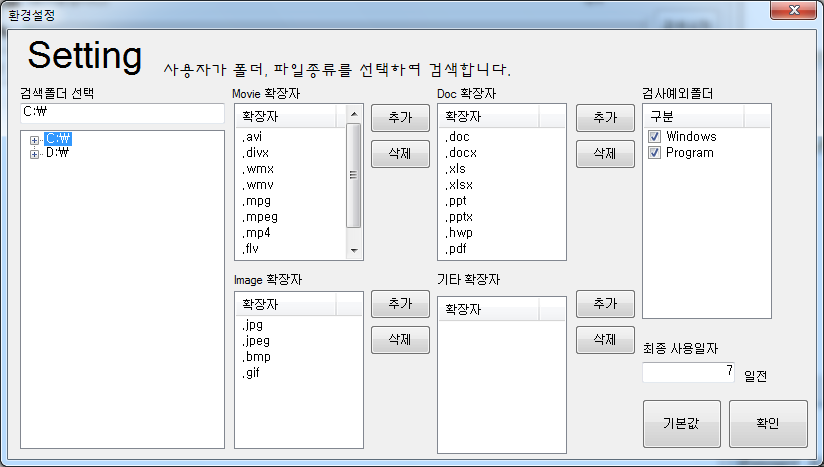
\includegraphics[width=0.7\textwidth]{Figures/Setting}
		\caption{환경설정}
		\label{fig:setting}
	\end{figure}

		\subsection{검색폴더 선택}
		모든 폴더 및 파일을 검색하는 것이 아닌 \textbf{일부분의 폴더에서 검색을 하고 싶을때 사용}한다. 하지만 다음 이미지와 같이 \textbf{Program Files 나 Windows 폴더}의 경우, 이후에 나올 \textbf{검색예외폴더 설정창에서 체크박스를 해제}하여야 검색이 가능하다.
		
		\begin{figure}[h]
			\centering
			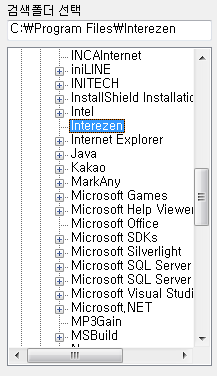
\includegraphics[height=0.35\textheight]{Figures/searchfolder}
			\caption{검색폴더 선택}
			\label{fig:searchfolder}
		\end{figure}
	
		\newpage
		
		\subsection{Movie 확장자}
		검색을 통해 메인 화면에 있는 동영상 섹션에 나열할 \textbf{동영상 파일들의 확장자를 나열해 놓은 칸}이다.
		우측의 \textbf{추가 버튼으로 동영상 섹션 내에서 검색하고 싶은 확장자를 더할 수 있으며 삭제 버튼으로 검색에서 제외하고 싶은 확장자를 제거} 할 수 있다.
		
		\begin{figure}[h]
			\centering
			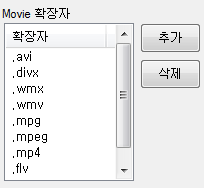
\includegraphics[width=0.4\textwidth]{Figures/Movie}
			\caption{Movie 확장자}
			\label{fig:movie}
		\end{figure}
	
		\subsection{Image 확장자}
		검색을 통해 메인 화면에 있는 이미지 섹션에 나열할 \textbf{이미지 파일들의 확장자를 나열해 놓은 칸}이다. 동영상 확장자 추가 버튼과 마찬가지로 우측의 \textbf{추가 버튼으로 이미지 섹션 내에서 검색하고 싶은 확장자를 더할 수 있으며, 삭제 버튼으로 검색에서 제외하고 싶은 확장자를 제거} 할 수 있다.
		
		\begin{figure}[h]
			\centering
			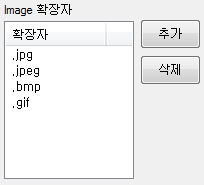
\includegraphics[width=0.4\textwidth]{Figures/Image}
			\caption{Image 확장자}
			\label{fig:image}
		\end{figure}
	
		\newpage
		
		\subsection{Doc 확장자}		
		검색을 통해 메인 화면에 있는 문서 섹션에 나열할 \textbf{문서 파일들의 확장자를 나열해 놓은 칸}이다. 동영상 확장자 추가 버튼과 마찬가지로 \textbf{우측의 추가 버튼으로 문서 섹션 내에서 검색하고 싶은 확장자를 더할 수 있으며, 삭제 버튼으로 검색에서 제외하고 싶은 확장자를 제거} 할 수 있다.
		
		추가적으로 문서 확장자의 대표적 예인 \textbf{.txt 확장자가 기본 확장자에 포함되어 있지 않기에 검색을 하기 위해선 추가 버튼을 이용하여 .txt 확장자를 추가}하여야 한다.
		
		\begin{figure}[h]
			\centering
			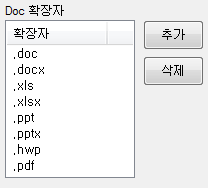
\includegraphics[width=0.4\textwidth]{Figures/Doc}
			\caption{Doc 확장자}
			\label{fig:Doc}
		\end{figure}
	
		\subsection{기타 확장자}
		검색을 통해 메인 화면에 있는 기타 섹션에 \textbf{검색하길 원하는 파일들의 확장자를 나열해 놓는 칸}이다. 동영상 확장자 추가 버튼과 마찬가지로 우측의 \textbf{추가 버튼으로 기타 섹션 내에서 검색하고 싶은 확장자를 더할 수 있으며, 삭제 버튼으로 검색에서 제외하고 싶은 확장자를 제거} 할 수 있다.
		
		추가적으로 \textbf{초기 기타 확장자 칸에는 아무런 확장자도 적혀 있지 않기에 사용자가 추가를 해주어야만} 관련 확장자 파일이 검색 된다.
		
		\begin{figure}[h]
			\centering
			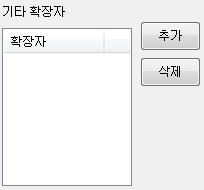
\includegraphics[width=0.4\textwidth]{Figures/etc}
			\caption{기타 확장자}
			\label{fig:etc}
		\end{figure}
	
		\newpage
	
		\subsection{검사예외폴더}	
		검사예외폴더 칸은 \textbf{검색시 소요되는 시간을 줄이기 위하여} 윈도우 운영체제와 대부분의 프로그램들이 설치되는 \textbf{ Windows 폴더와 Program Files 폴더를 체크박스를 통해 검색에서 제외하거나 포함}시키는 것이 가능하다.
		
		검사예외폴더 칸에는 기본적으로 \textbf{Windows와 Program 폴더만이 지정 가능}하다.
		
		\begin{figure}[h]
			\centering
			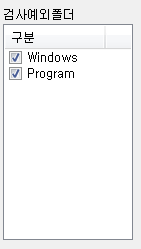
\includegraphics[width=0.4\textwidth]{Figures/except}
			\caption{검사예외폴더}
			\label{fig:except}
		\end{figure}
	
		\newpage
	
		\subsection{최종 사용일자}	
		최종 사용일자 칸은 검색 시 나열할 파일이 \textbf{최종 사용일자 칸에 적힌 날짜 이전의 사용 파일만}을 출력하는 일종의 조건문이다.
		
		사용 날짜에 상관없이 모든 파일을 출력을 하고 싶을때는 최종 사용일자를 0 일전으로 적으면 된다.
		
		\begin{figure}[h]
			\centering
			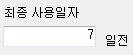
\includegraphics[width=0.4\textwidth]{Figures/date}
			\caption{최종 사용일자}
			\label{fig:date}
		\end{figure}
	
		\newpage
	
		\subsection{기본값 \& 확인}
		기본값 버튼은 확장자를 추가하거나 삭제 등으로 \textbf{변경사항이 생겼을 경우 프로그램에 내장 된 변경 전의 초기값}으로 돌아가게 된다. 또한 기본값은 현재 변경이 불가능하다.
		
		확인 버튼의 경우 \textbf{현재까지 변경한 내용을 저장}하기 위한 버튼이다.
		
		\begin{figure}[h]
			\centering
			\includegraphics[width=0.4\textwidth]{Figures/button}
			\caption{기본값 \& 확인}
			\label{fig:button}
		\end{figure}
	
	\clearpage
	\section{CapacityManger Bug and Improvement}

		
		\LARGE \bf |Bug| \newline
		
		\begin{enumerate}
		\large \item 한번에 전체 선택이 불가능 \newline
		
		\item 환경설정에서 폴더 선택하고 나갔다가 다시 환경설정 들어가면
		선택한 폴더위치가 초기화되버림 \newline
		
		\item 파일명, 파일크기, 마지막사용 날짜별 정리 기능 없음 \newline
		
		\item 환경설정에 폴더 설정 부분 복잡성 \newline
		
		\item 검색 시간이 오래 걸리거나 검색이 마무리 되지 않을 때가 있음
		('폴더 취합 중'이 오래 걸림) \newline \newline
		
	\end{enumerate}
		
		\begin{figure}[h]
			
			\centering
			
			\includegraphics[height=0.35\textheight]{Figures/"Long Time(Bug)"}
			
			\caption{취합 중 멈춤}
			
			\label{fig:long-time}
			
		\end{figure}
		
		\newpage
		
		\bf \LARGE |Improvement| \newline
		
		\begin{enumerate}
		
		\large \item 몇일 이상 미사용 파일 삭제 기능 \newline
		
		\item 파일 이름으로 검색 기능 \newline
		
		\item 디스크 정리 기능 \newline
		
		\item 최근에 사용한 파일들 보여주기 \newline
		
		\item 자주 사용하는 폴더 보여주기 \newline
		
		\item 전체 선택 기능(다중 선택은 가능하지만 한번에 전체 선택 기능 없음) \newline
		
		\item 파일명, 파일크기, 마지막사용 날짜별 정리 기능
		\end{enumerate}
\end{document}